\documentclass{scrartcl}

\usepackage[utf8]{inputenc}
\usepackage{color}
\usepackage{xcolor}

\usepackage{graphics}           % Add pictures to the document
\usepackage{graphicx}           % Add pictures to the document
\usepackage{subfigure}          % 2 pictures side by side

\title{Dokumentation ProductAR}
\author{Maximilian Rehberger}
\date{\today}

\setcounter{secnumdepth}{4}
\setcounter{tocdepth}{4}

\definecolor{darkcerulean}{rgb}{0.03, 0.27, 0.49}
\definecolor{frenchblue}{rgb}{0.0, 0.45, 0.73}
\definecolor{babyblueeyes}{rgb}{0.63, 0.79, 0.95}

\addtokomafont{section}{\color{darkcerulean}}
\addtokomafont{subsection}{\color{frenchblue}}
\addtokomafont{subsubsection}{\color{babyblueeyes}}

\graphicspath{ {./img/} }                % Path to images

\begin{document}


\maketitle

\newpage


\renewcommand*\contentsname{}
\section{Inhaltsverzeichnis}
\tableofcontents{}


\newpage

\section{Einleitung}

\subsection{Zweck}

Produkte können zum Beispiel beim Einkaufen mit dem Smartphone gescannt werden und erkannt werden. Informationen werden angezeigt wie zum Beispiel Bilder oder ein Preisvergleich. Mithilfe der App soll man einen Barcode einscannen können und Informationen zu den Produkten erhalten. Weiterhin kann der Nutzer ein Produkt in Augmented Reality (AR) testen und sieht somit wie es in Wirklichkeit aussehen wird, wenn er es kaufen würden.

\newpage

\section{Allgemeine Übersicht}

\subsection{Beschreibung Ausgangssituation}

Es gibt bereits viele Shopping-Apps wie zum Beispiel Ikea, H\&M oder S'Oliver. Das Problem ist, dass jeder am Ende für jedes Geschäft eine eigene App auf dem Smartphone hat. Diese App soll die Möglichkeiten geben mehrere unterschiedliche Produkte in einer App zu speichern und zu verwalten. Also eine App für alle Produkte.

\subsection{Produkteinsatz}

 Die App kann zum Beispiel als Einkaufsliste oder Wunschliste für Produkte eingesetzt werden.
 Darüber hinaus bieten sich noch viele weitere Möglichkeiten.

\subsection{Produktumfeld}

Die App wird hauptsächlich im privaten Umfeld umgesetzt, beim Einkaufen in Geschäften oder Online-Einkauf.

\subsection{Produktfunktionalität}

Scannen von Produkten, Informationen zu Produkten, Preisvergleich, Bilder hochladen für Produkte, Produkte in AR testen.

\subsection{Personas}

\subsubsection{Nutzer}

\subsubsection{Verkäufer}

\subsubsection{Admin}


\newpage

\section{Architekturkonzept und Entwurf}

\subsection{Ursprüngliches Architekturkonzept}

\begin{figure}[h]
\centering
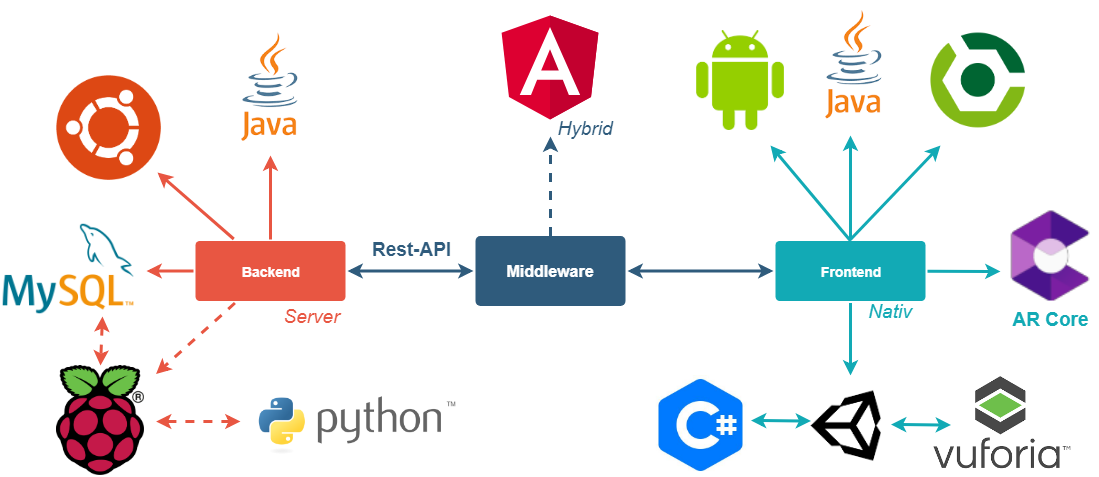
\includegraphics[width=380px]{img/Architekturkonzept.png}
\caption{Ursprüngliches Architekturkonzept}
\end{figure}

\subsection{Aktualisiertes Architekturkonzept}

\begin{figure}[h]
\centering
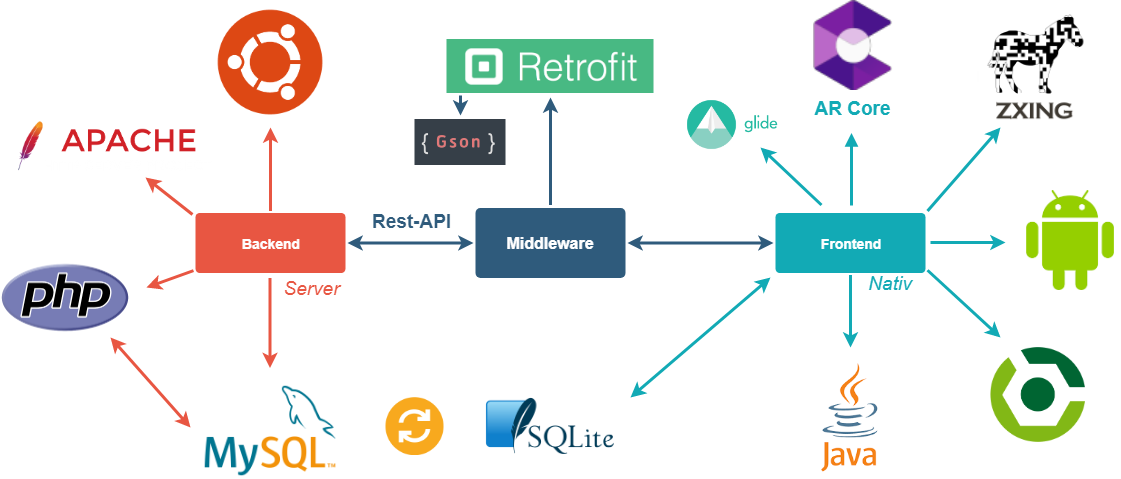
\includegraphics[width=380px]{img/ArchitekturkonzeptNew.png}
\caption{Aktualisiertes Architekturkonzept}
\end{figure}

\newpage

\subsection{Anfängliche Skizze Datenbankentwurf}

\subsubsection{MySQL Datenkbank (Remote)}

Ursprünglich war geplant, dass die Daten ausschließlich auf dem Server in einer MySQL Datenbank gespeichert werden.

\begin{figure}[h]
\centering
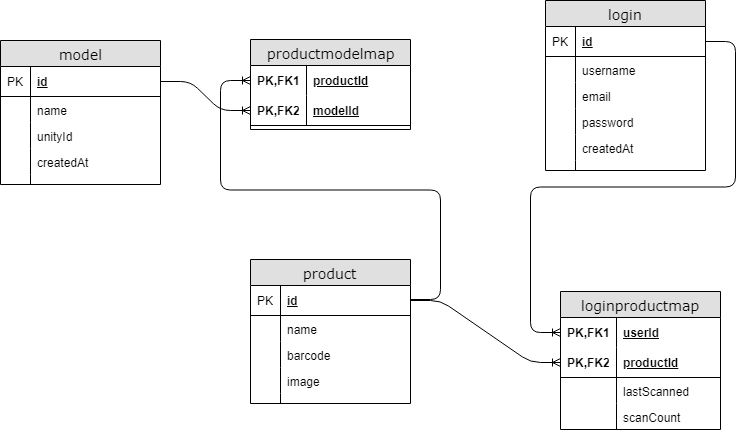
\includegraphics[width=380px]{img/Skizze_Datenbank_1.png}
\caption{Anfängliche Skizze Datenbankentwurf}
\end{figure}

\newpage

\subsection{Anfängliche Skizze Java Klassen}

\begin{figure}[h]
\centering
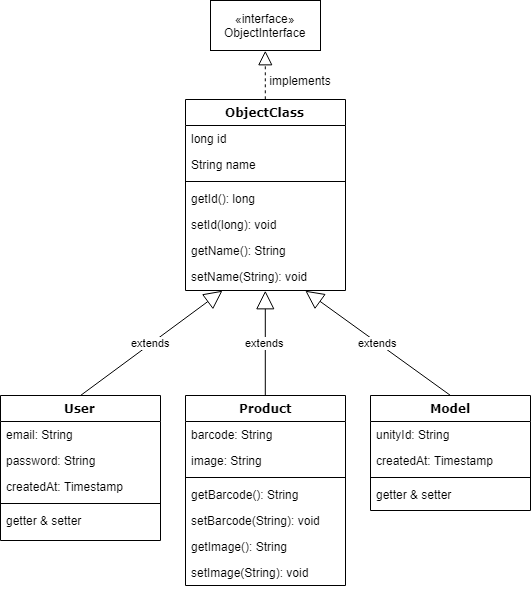
\includegraphics[width=320px]{img/Skizze_Java_1.png}
\caption{Anfängliche Skizze Datenbankentwurf}
\end{figure}

\newpage

\subsection{Endgültige Skizze Datenbankentwurf}

\subsubsection{SQLite Datenbank (Lokal)}

\begin{figure}[h]
\centering
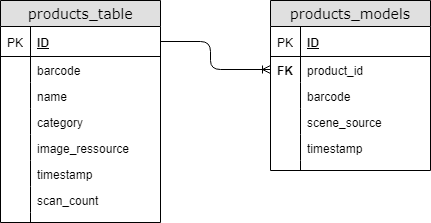
\includegraphics[width=180px]{img/Skizze_Datenbank_SQLite.png}
\caption{Skizze Datenbankentwurf: SQLite}
\end{figure}

\subsubsection{MySQL Datenbank (Remote)}

\begin{figure}[h]
\centering
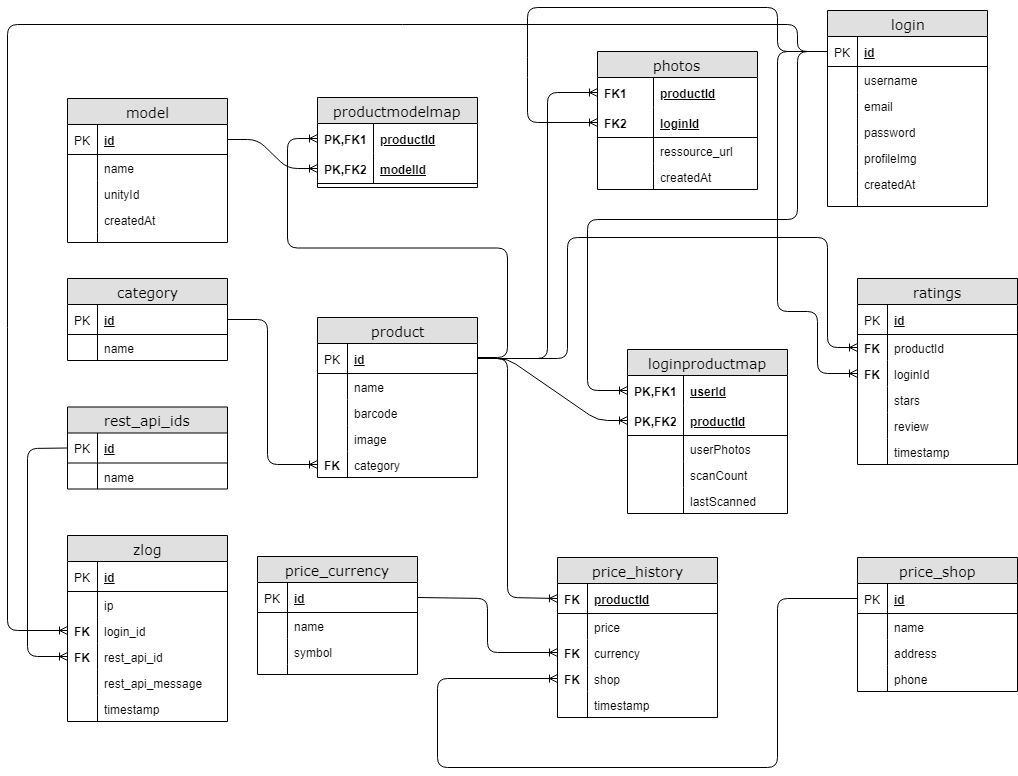
\includegraphics[width=380px]{img/Skizze_Datenbank_2.png}
\caption{Aktualisierte Skizze Datenbankentwurf: MySQL}
\end{figure}

\newpage

\subsection{Endgültige Skizze Java Klassen}

\begin{figure}[h]
\centering
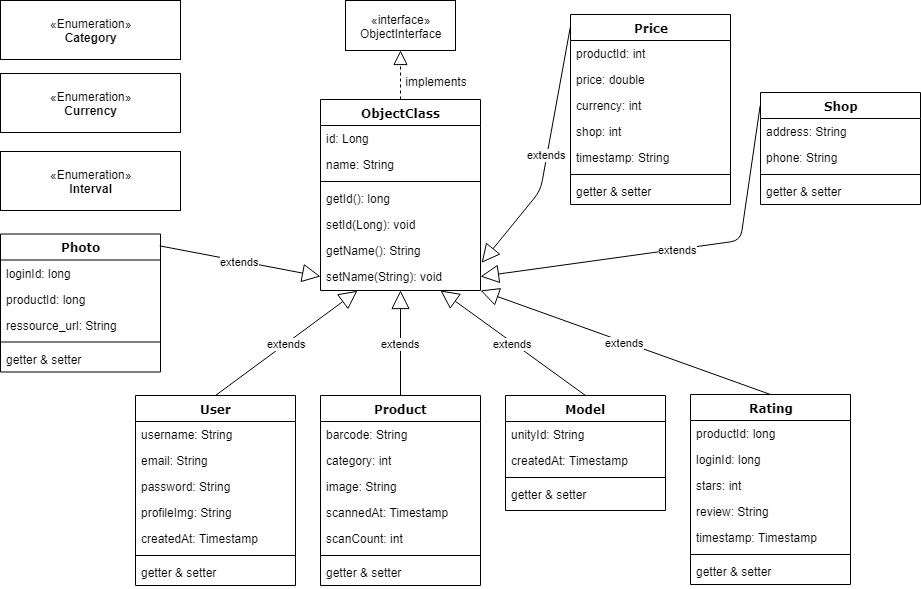
\includegraphics[width=380px]{img/Skizze_Java_New.png}
\caption{Aktualisierte Skizze: Java Klassen}
\end{figure}

\subsection{Übersicht Backend Server}

Der Backend Server ist ein gemieteter Server von Hosteurope. \newline
Produktbezeichnung: "Virtual Server Linux Advanced 8.2". \newline
Dieser hat folgende Linux Version installiert: Ubuntu 16.04.6 LTS. \newline \newline

\noindent Die Technischen Spezifikationen lauten wie folgt: \newline 

\noindent 4 virtuelle Kerne \newline
\noindent 6 GB RAM \newline 
\noindent 200GB SSD \newline 

\noindent Es handelt sich hierbei um einen virtuellen Server, das bedeutet, dass sich der Server mit anderen "Containern" die Hardware eines Servers teilen. % Die Hardware eines großen Server wird auf die Container entsprechend aufgeteilt. % 
\newline

\noindent Der Server hat eine eigene Domain: www.nimoo.de. 

\newpage

\subsection{Übersicht REST API}

Die Rest Schnittstelle wurde mit PHP auf dem Webserver umgesetzt welcher vom Backend Server bereits zur Verfügung gestellt wurde. 
Für jede Ressource existiert ein Pfad, mit entsprechender PHP Datei. \newline 

\noindent Der Hauptpfad für die App auf dem Webserver: "https://www.nimoo.de/apps/productar" \newline

\noindent Folgende Pfade existieren auf dem Webserver: \newline

\noindent ../products/ \newline
\noindent ../products/images/ \newline
\noindent ../products/photos/ \newline
\noindent ../products/prices/ \newline
\noindent ../products/ratings/ \newline
\noindent ../users/ \newline
\noindent ../users/images \newline
\noindent ../models/ \newline

\subsection{Technische Entscheidungen}

\subsubsection{Warum Android?}

Die Entscheidung, die App für Android zu entwickeln wurde getroffen, da Android zumindest in Deutschland einen höheren Marktanteil besitzt als iOS. Vor allem die Studenten der Fakultät Informatik und Wirtschaftsinformatik (FIW) und in der Vertiefung Mobile Solutions benutzen mehrheitlich Android Smartphones. Ein weiterer Grund ist, dass Android Java basiert ist und dafür sehr gut geeignet ist, wenn bereits fortgeschrittene Erfahrungen mit der Programmiersprache Java gegeben sind. Weiterhin gibt es beim Entwickeln keine Mehrkosten, da es bereits viele Open-Source Erweiterungen (Bibliotheken) gibt und Anleitungen, die das Entwickeln weiter vereinfachen.

\subsubsection{Welche Androidversion?}

Als minimal unterstützte Android Version (minSdkVersion) für die App musste die Api 24 (Android 7) verwendet werden. Dies liegt daran, dass die AR Funktionialität mit der Google AR Core Erweiterung erst ab Android Version 7 (Api 24) unterstützt wurde und alle vorherigen Versionen keine Unterstützung haben. Dies hat den Nachteil, dass nur ca. 37,1 \% aller Android Geräte unterstützt werden im Vergleich zu den 95,3 \% die mit Android 4.4 (Api 19) unterstützt würden. 

\subsubsection{Welche Entwicklungsumgebung?}

Zum Entwickeln der App wurde hauptsächlich die Entwicklungsumgebung von Android Studio und IntelliJ genutzt.

\subsubsection{Wieso Google AR Core?}

Googles neuestes Framework für Augmented Reality Anwendungen heist "AR Core". Im Vergleich zu einer AR Anwendung mit Unity lässt es es sich sehr einfach in die App integrieren (Als Fragment oder View in der Aktivity). Weiterhin lassen sich Modelle (.OBJ) sehr einfach mit dem Sceneform Plugin einbinden und bearbeiten. 

\subsubsection{Wieso eine MySQL Datenbank?}

Zum einen war die MySQL Datenbank ebenfalls schon auf dem Backend Server aufgesetzt, somit war keine weitere Konfiguration notwendig. Weiterhin ist es sehr einfach eine Datenbank mit SQL zu erstellen und Abfragen durchzuführen.

\subsubsection{Wieso eine REST API?}

Die Rest API ist die Schnittstelle zwischen der App und der Datenbank auf dem Server. Diese wird benötigt, da man aus Sicherheitsgründen keine direkte Verbindung zwischen App und Datenbank zulassen darf.

\subsubsection{Vergleich mit Alternativlösungen}

\paragraph{Firebase von Google}.\newline

\noindent Die Backendlösung von Google ist "FireBase" und wäre erheblich einfacher umzusetzten und hätte ebenfalls den Vorteil, dass kein externer Server benötigt wird. Warum wurde diese Lösung in diesem Projekt jedoch nicht verwendet? Die Datenbank enthält sensible Daten, wie zum Beispiel Nutzerdaten. Diese sollen nicht an Google gesendet werden.

\paragraph{Alternative Datenbankmodelle}.\newline

\noindent PostgreSQL und MongoDB.

\newpage

\section{Technische Dokumentation}

\subsection{Android Manifest}

\subsection{Java Interfaces}

\subsubsection{ObjectInterface}

\subsubsection{ScanResultReceiver}

\subsubsection{IRetrofitCRUD}

\subsubsection{JsonPlaceHolderApi}

\subsection{Java Klassen}

\subsubsection{Objekt Klassen}

\paragraph{Object Class (Abstract)}

\paragraph{Product}

\paragraph{User}

\paragraph{Model}

\paragraph{Photo}

\paragraph{Price}

\paragraph{Shop}

\paragraph{Category (Enum)}

\paragraph{Currency (Enum)}

\paragraph{Interval (Enum)}

\subsubsection{Aktivity Klassen}

\paragraph{MainActivity}

\paragraph{SplashScreen}

\paragraph{ProductArActivity}

\paragraph{ProductScanActivity}

\paragraph{CaptureActivityPortrait}

\paragraph{LastScannedProductsActivity}

\paragraph{CreateProductActivity}

\paragraph{ProductDetailActivity}

\paragraph{ProductPhotoGalleryActivity}

\paragraph{ProductPhotoDetailActivity}

\paragraph{CreatePriceActivity}

\paragraph{PriceHistoryActivity}

\paragraph{RegisterActivity}

\paragraph{LoginActivity}

\paragraph{ProfileActivity}

\paragraph{SettingsActivity}

\paragraph{InfoActivity}

\subsubsection{Adapter Klassen}

\paragraph{ProductListAdapter}

\paragraph{PhotoAdapter}

\subsubsection{Hilfs Klassen}

\paragraph{GeneralHelper}

\paragraph{BarcodeHelper}

\paragraph{QRCodeHelper}

\paragraph{LoginHelper}

\paragraph{SettingsHelper}

\paragraph{ImageHelper}

\paragraph{PhotoHelper}

\paragraph{UploadHelper}

\paragraph{PriceHelper}

\subsubsection{Fragment Klassen}

\paragraph{ScanFragment}

\paragraph{CustomArFragment}

\subsubsection{Retrofit Schnittstelle}

\subsubsection{Network Monitor}

\subsubsection{Background Service}

\subsubsection{Notifications}

\subsection{Ressourcen}

\subsubsection{Layout}

\subsubsection{Drawable Icons}

\subsubsection{App Icon}

\subsubsection{Animation}

\subsubsection{Menu}

\subsubsection{Assets}

\subsubsection{Values}

\subsection{Rest Api}


\newpage

\section{Veröffentlichung im Google Play Store}

\subsection{Store Eintrag}

\subsection{Alpha Test}

\subsection{Beta Test}


\newpage

\section{Zukünftige Entwicklungen}


\newpage

\section{Fazit}


\newpage

\section{Verwendete Technologie, Frameworks und Software}


\newpage

\section{Verlinkung Repositories}


\newpage

\section{Verlinkung Tutorials}


\newpage

\section{Quellenangabe}


\end{document}
